\section{システム実装}
\subsection{チーム構成と役割分担}
本プロジェクトは，6名(近藤・関屋・岩波・須磨・木村・仲里)のチームで実施した．
本システムでは，同期通信機能・楽器音源の生成・再生機能・人形の物理演出機能の3つの機能が必要であり，チームメンバはそれぞれの担当を分担した．
このチームでは，機能ごとにタスクを担当するのではなく，細かい成果物ごとに担当を分担する方式を採用した．
特に，ProcessingやArduinoといったプログラムはハッカソン1の学生が主体となり，ハッカソン2の学生に
そのレビュー及び，手の回らない部分の実装を依頼するという形で，チーム内での役割分担を行った．
なお，本システムのサーバおよびクライアントはいずれもArduinoで実装されており，主要な関数は
サーバ側とクライアント側に分けられる．

\vspace{1zh}\noindent
\textbf{［サーバ側］}

\textbf{Bar\_control()関数}\quad 小節番号を送信する関数である．前回の送信から一定の間隔が経過するたびに
小節番号を1つ進め，その値をUDPでブロードキャスト送信する．小節番号は0から39までの範囲で循環させる．
フローチャートを図\ref{fig:bar_control}に示す．

\textbf{BPM\_control()関数}\quad テンポを変更する関数である．テンポを増減する2つのスイッチの押下を検出し，
上限・下限の範囲内でテンポを5ずつ増減させる．テンポの変更後，最後にスイッチが押されてから一定時間が
経過した時点で，変更後のテンポをUDPで送信する．これにより，スイッチを連続して押した場合でも送信が
1回にまとめられる．フローチャートを図\ref{fig:bpm_control}に示す．

\textbf{detectPress()関数}\quad スイッチの押下を検出する関数である．スイッチの読み値には接点の機械的な
振動によるチャタリングが生じるため，読み値が一定時間安定して初めて状態の変化を確定する．これにより，
1回の押下が複数回として誤検出されることを防ぐ．フローチャートを図\ref{fig:detect_press}に示す．

\vspace{1zh}\noindent
\textbf{［クライアント側］}

\textbf{Parse\_data()関数}\quad 受信データの種別を判別する関数である．サーバから送られる1バイトのデータは
小節番号とテンポのいずれかであり，その値が一定値以上であればテンポ，それ未満であれば小節番号として扱う．
小節番号の場合は，各クライアントに固有のオフセットを加えて自身の演奏位置を求める．フローチャートを
図\ref{fig:parse_data}に示す．

\textbf{BPM\_update()関数}\quad テンポから演奏の時間基準を求める関数である．テンポを受信した際に，
基準となる4分音符の長さをミリ秒単位で算出し，以降の演奏タイミングの基準とする．フローチャートを
図\ref{fig:bpm_update}に示す．

\textbf{Performance()関数}\quad 演奏を進める関数である．受信した小節番号に対応する音符を，あらかじめ
保持している譜面データから先頭から順に読み出す．各音符の周波数，発音する長さ，強さ，およびテンポを
シリアル通信でProcessingへ送信し，音符の長さに応じた間隔をおいて次の音符へ進む．フローチャートを
図\ref{fig:performance}に示す．

% ===== サーバ側 =====
\begin{figure}[H]
  \begin{center}
    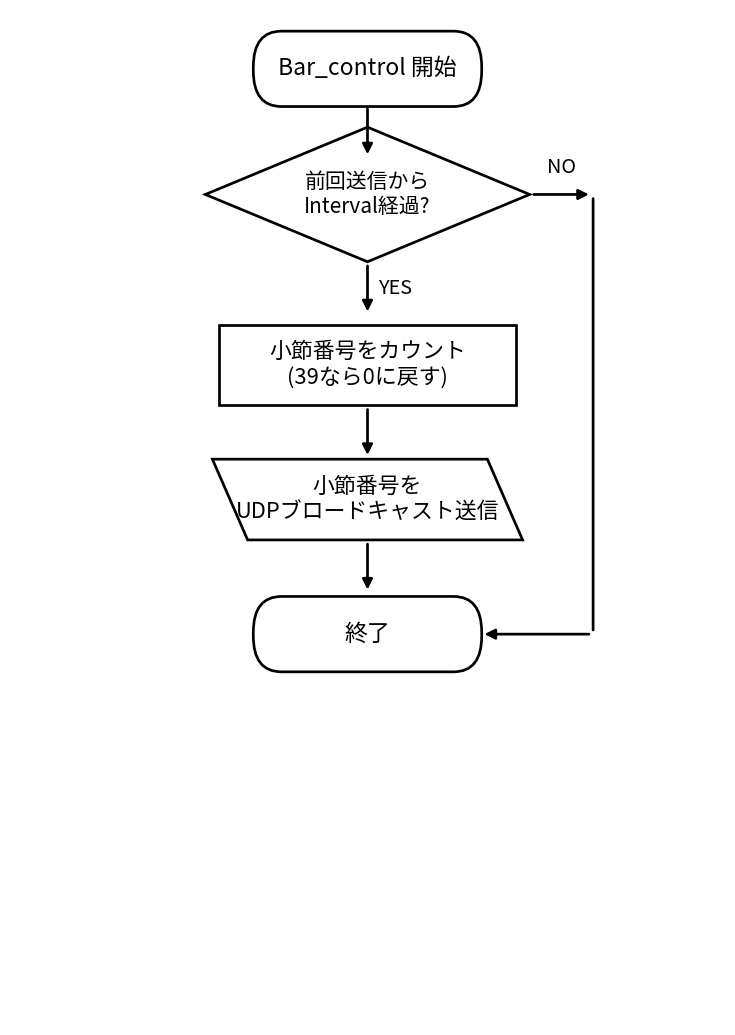
\includegraphics[width=0.55\linewidth]{fig/fc_bar_control.png}
  \end{center}
  \caption{Bar\_control()関数のフローチャート}
  \label{fig:bar_control}
\end{figure}

\begin{figure}[H]
  \begin{center}
    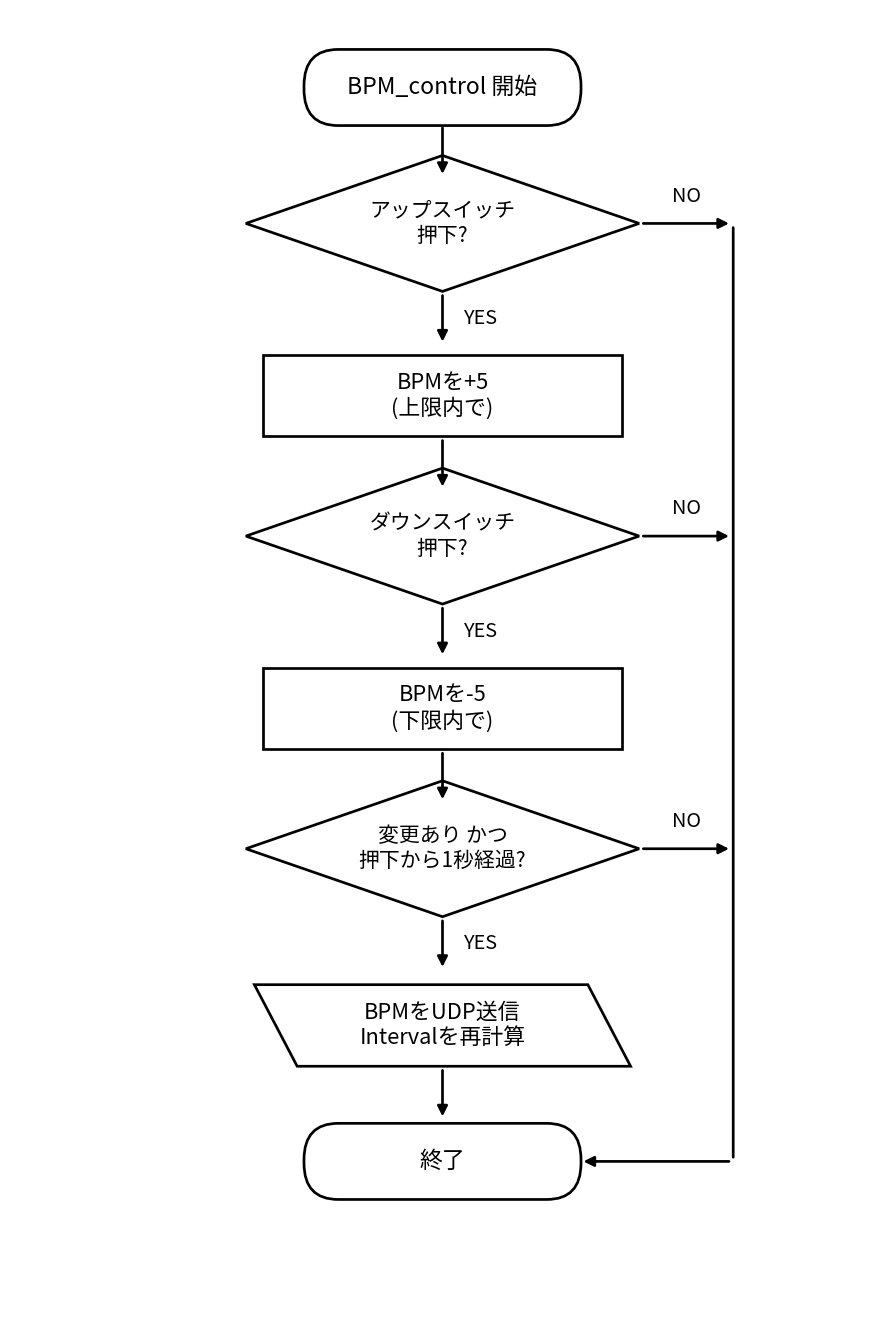
\includegraphics[width=0.6\linewidth]{fig/fc_bpm_control.png}
  \end{center}
  \caption{BPM\_control()関数のフローチャート}
  \label{fig:bpm_control}
\end{figure}

\begin{figure}[H]
  \begin{center}
    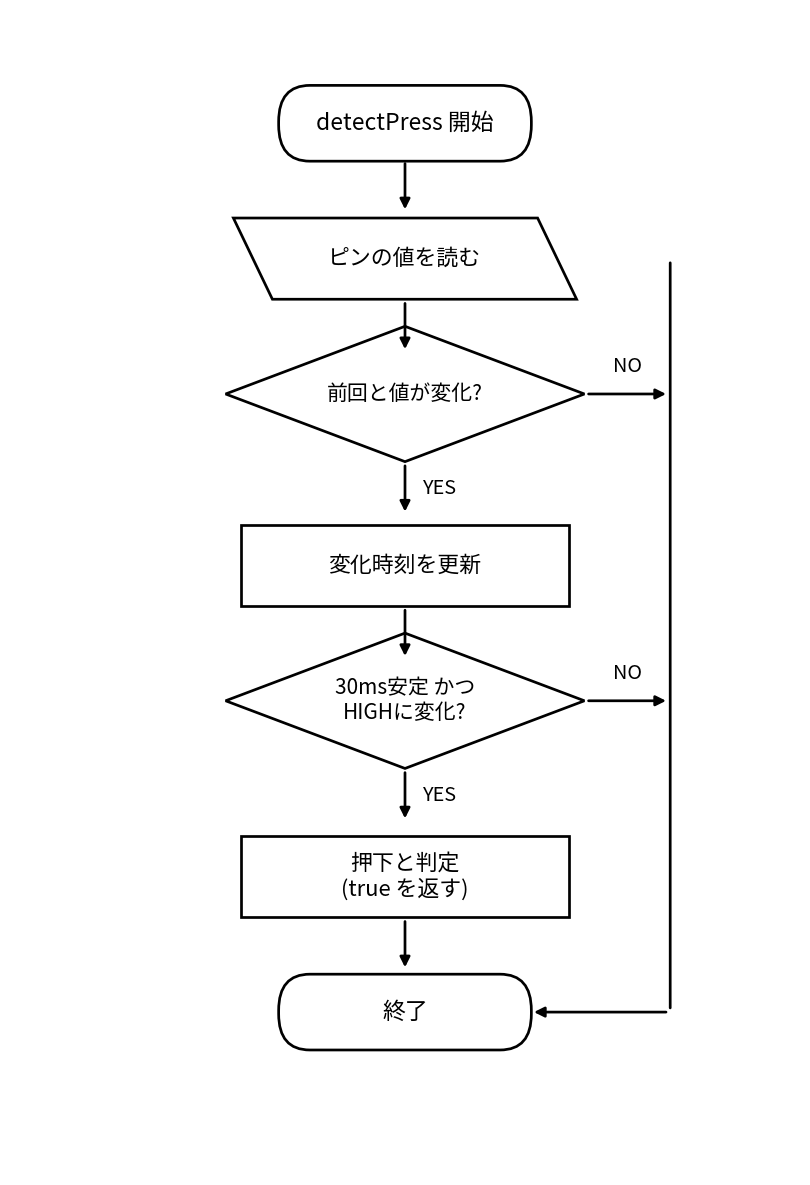
\includegraphics[width=0.55\linewidth]{fig/fc_detect_press.png}
  \end{center}
  \caption{detectPress()関数のフローチャート}
  \label{fig:detect_press}
\end{figure}

% ===== クライアント側フローチャート =====
\begin{figure}[H]
  \begin{center}
    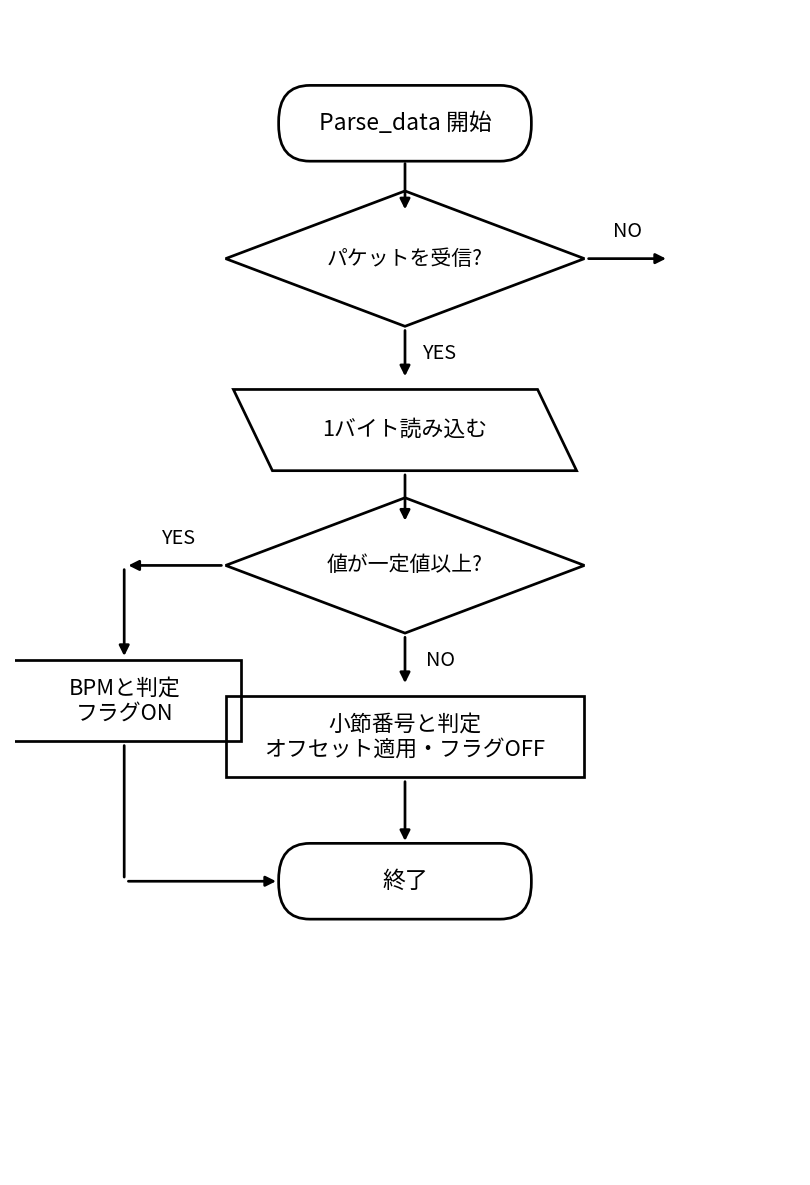
\includegraphics[width=0.55\linewidth]{fig/fc_parse_data.png}
  \end{center}
  \caption{Parse\_data()関数のフローチャート}
  \label{fig:parse_data}
\end{figure}

\begin{figure}[H]
  \begin{center}
    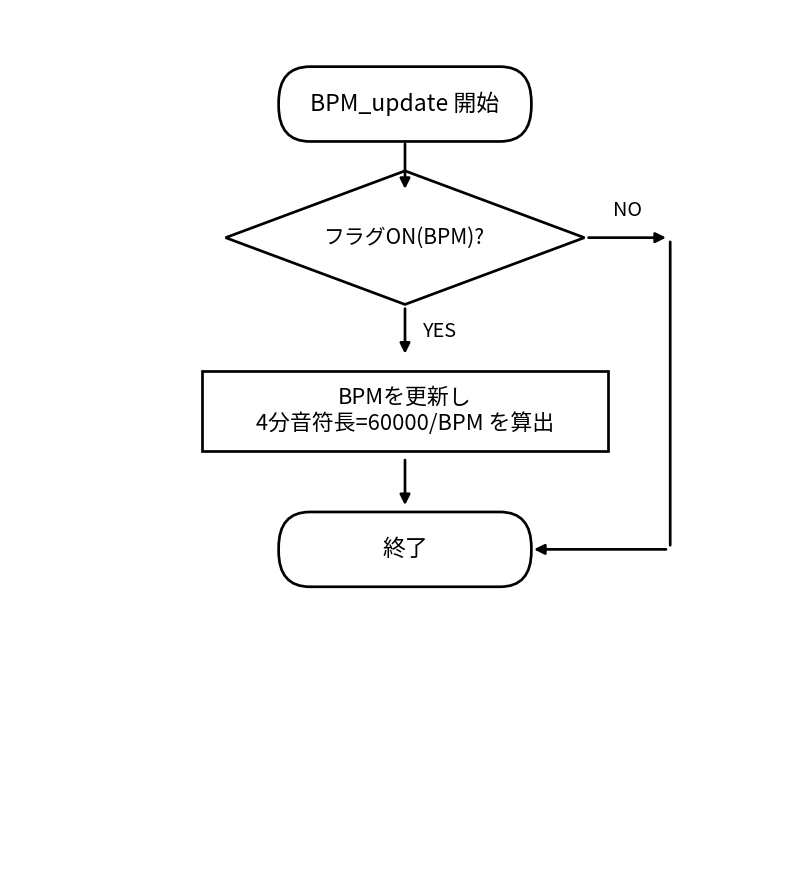
\includegraphics[width=0.5\linewidth]{fig/fc_bpm_update.png}
  \end{center}
  \caption{BPM\_update()関数のフローチャート}
  \label{fig:bpm_update}
\end{figure}

\begin{figure}[H]
  \begin{center}
    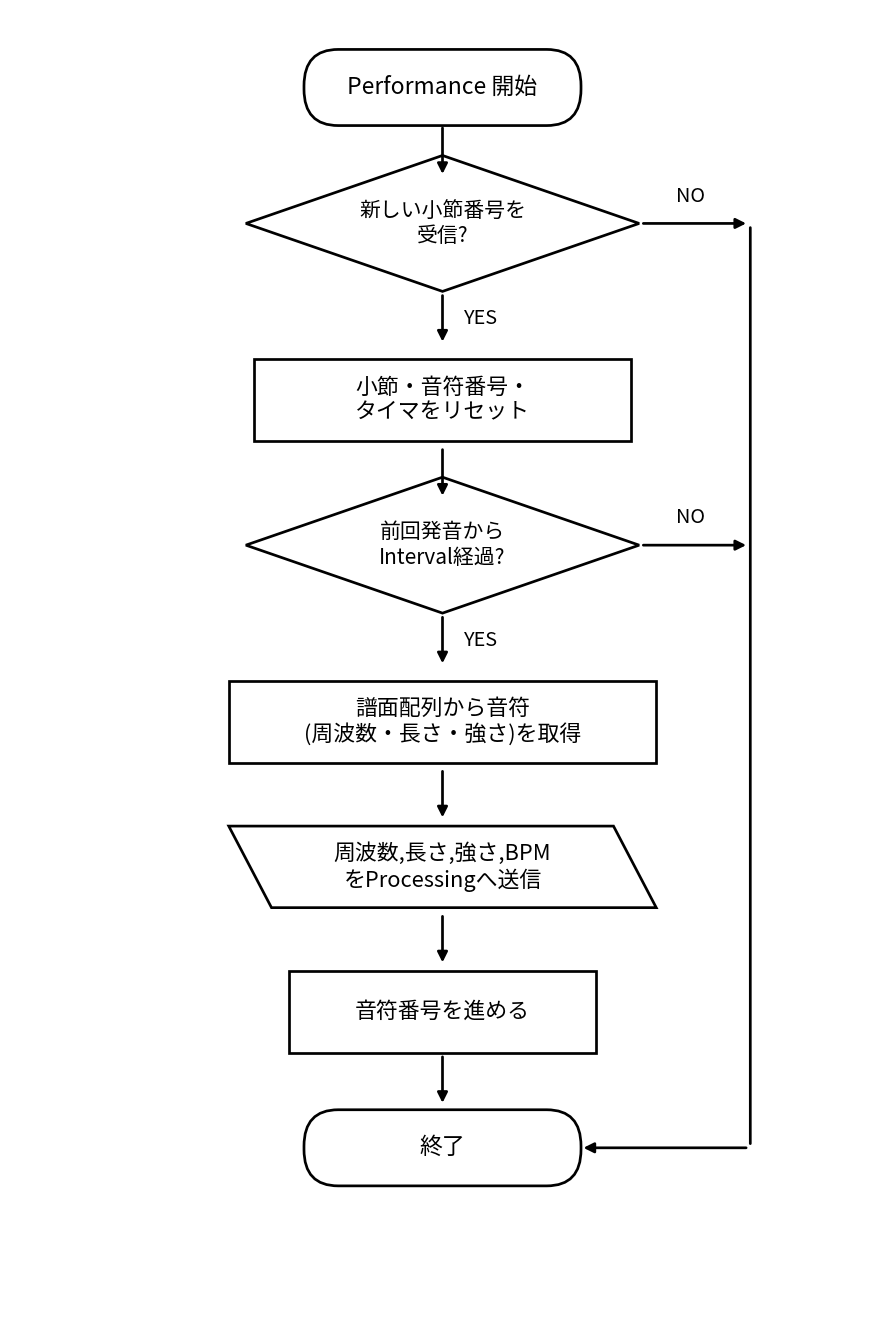
\includegraphics[width=0.55\linewidth]{fig/fc_performance.png}
  \end{center}
  \caption{Performance()関数のフローチャート}
  \label{fig:performance}
\end{figure}


\begin{figure}[H]
    \begin{center}
    \resizebox{\linewidth}{!}{%
    \begin{ganttchart}[y unit title=0.4cm,
    y unit chart=0.5cm,
    vgrid,hgrid,
    title label anchor/.style={below=-1.6ex},
    title left shift=.05,
    title right shift=-.05,
    title height=1,
    title/.append style={fill=yellow!10},
    progress label text={},
    bar height=0.7,
    group right shift=0,
    group top shift=.6,
    group height=.3]{1}{24}
    %labels
    \gantttitle{8 Weeks}{24} \\
    \gantttitle{W1}{3}
    \gantttitle{W2}{3}
    \gantttitle{W3}{3}
    \gantttitle{W4}{3}
    \gantttitle{W5}{3}
    \gantttitle{W6}{3}
    \gantttitle{W7}{3}
    \gantttitle{W8}{3}\\
    %===== 実装フェーズ =====
    \ganttgroup{実装フェーズ}{2}{17} \\
    \ganttbar[bar/.append style={fill=blue!35}]{サーバ・クライアント実装（仲里・岩波）}{2}{11} \\
    \ganttbar[bar/.append style={fill=green!35}]{ピアノ音源（木村）}{2}{9} \\
    \ganttbar[bar/.append style={fill=red!55}]{トロンボーン音源（近藤）}{2}{9} \\
    \ganttbar[bar/.append style={fill=green!35}]{ヴァイオリン音源（仲里）}{9}{15} \\
    \ganttbar[bar/.append style={fill=red!55}]{カスタネット音源（近藤）}{9}{14} \\
    \ganttbar[bar/.append style={fill=orange!40}]{サーボ駆動・エンタメ（木村・関屋）}{2}{17} \\
    \ganttbar[bar/.append style={fill=red!55}]{トロンボーン・カスタネット人形製作（近藤 他）}{11}{16} \\
    \ganttbar[bar/.append style={fill=gray!30}]{ステージ製作（須磨・岩波）}{14}{22} \\
    %===== テストフェーズ =====
    \ganttgroup{テストフェーズ}{5}{24} \\
    \ganttbar[bar/.append style={fill=red!55}]{各楽器の音確認・演奏テスト（近藤・木村・仲里）}{5}{24} \\
    \ganttbar[bar/.append style={fill=gray!30}]{同期・エンタメ動作テスト（仲里・木村・関屋・岩波）}{11}{22} \\
    \ganttbar[bar/.append style={fill=red!55}]{演奏テスト（全員）}{18}{24}
    \end{ganttchart}%
    }
    \end{center}
    \caption{開発スケジュール}
    \label{gantt1}
\end{figure}
図\ref{gantt1}に，開発スケジュールを示す．
まず，サーバー・クライアントの実装は仲里・岩波が担当し，サーバーの同期通信機能を実装した．
次に，Processing上での楽器音源の生成は，それぞれトロンボーンとカスタネットの音色作成を近藤が担当し，ピアノの音色作成を木村が担当した．ヴァイオリンの音色作成は仲里が担当した．
人形のサーボモータ駆動を含むエンタメ部分の実装は木村・関屋が主に担当し，後に人形の
サーボモータ接合部の実装は近藤と仲里で手伝った．
人形を配置するステージの作成は須磨・岩波が担当した．
テストフェーズでは，各楽器の音確認・演奏テストを近藤・木村・仲里が担当し，サーボモータの動作確認テストは木村と関屋が主に担当した．
同期テストはサーバとクライアントの実装を行った仲里と岩波が担当し，最終的な演奏テストは
全員で実施した．

\subsection{報告者の担当範囲と技術的課題}
報告者は，トロンボーンおよびカスタネットの音源をProcessing上で実装した．
他にも後付の作業として人形作成が加わったが，そちらは物理的な作業であり，報告者の専門分野ではないため，本報告書では主に音源の実装について書く．
音源は，クライアントから送信される音符の周波数をもとに，Minimライブラリを用いて波形を合成することで生成する．

トロンボーンの音源を実装するにあたり，まず単純な波形を用いて音を合成した．しかし，矩形波や
単一のオシレータ(一定周期の波形を出力する発振器)による波形では，生成される音は電子的なブザー音のように聞こえ，実際のトロンボーンの
音とは大きく異なるものであった．実物のトロンボーンは，基本周波数に加えて多くの倍音を含み，また
音の立ち上がりや減衰にも特有の変化を持つ．単純な波形ではこれらの特徴が再現されないため，
トロンボーンらしい音色を得ることが課題となった．

カスタネットは，トロンボーンとは異なる種類の課題を持つ．実際のカスタネットの音の波形を
図\ref{fig:castanet_real}に示す．図から，打撃の瞬間に振幅が最大となり，その後急速に減衰していること，
および波形が正弦波のような規則的な周期を持たず，不規則に振動していることが読み取れる．
\begin{figure}[H]
  \begin{center}
    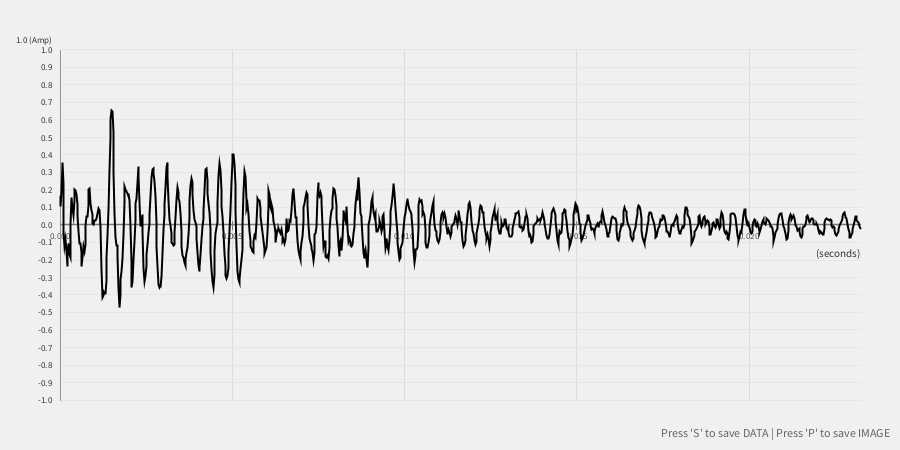
\includegraphics[width=0.8\linewidth]{fig/castanet_real.png}
  \end{center}
  \caption{実際のカスタネットの音の波形}
  \label{fig:castanet_real}
\end{figure}
一方，オシレータは周期的な波形を出力するため，明確な基本周波数を持ち，音程のある音として知覚される．
これは，図\ref{fig:castanet_real}に示したカスタネットの不規則な波形とは根本的に異なる．そのため，
音程を持たず，不規則な打撃音として聞こえるカスタネットの音を，オシレータを基本とするMinimの枠組みで
いかに合成するかが課題となった．

\subsection{予備実験と設計値の決定}
音源の各パラメータは，実測から一意に定まるものではなく，実際の楽器の音に近い聴感が得られるように
調整して決定する必要がある．そこで，Processing上で合成音の波形および周波数成分を確認しながら，
実際の楽器音と聴き比べる予備実験を繰り返し，各設計値を決定した．

トロンボーンの音源では，波形テーブルの倍音構成に加え，音色を整えるためのフィルタおよびエンベロープの
パラメータを調整した．波形テーブルには高次の倍音まで含まれており，そのままでは電子的で硬い音となる．
そこで，遮断周波数1200\,Hzのローパスフィルタを適用し，高域成分を抑えることで管楽器らしい柔らかい音色に
近づけた．また，音の立ち上がりが急峻すぎると機械的な印象となるため，立ち上がり時間を0.08\,秒，減衰時間を
0.05\,秒，持続レベルを0.8，余韻を0.3\,秒とするエンベロープを設定し，管楽器の発音に近い緩やかな立ち上がりと
した．さらに，発音直後に基準周波数の0.96倍から0.12\,秒かけて基準周波数へ移行させることで，金管楽器に
みられる発音時のわずかなピッチの揺れを再現した．設計値を表\ref{tab:trombone_params}に示す．これらの値は
合成音を試聴しながら段階的に決定した．

\begin{table}[H]
  \centering
  \caption{トロンボーン音源の設計値}
  \label{tab:trombone_params}
  \begin{tabular}{ll}
    \hline
    パラメータ & 設計値 \\
    \hline
    ローパスフィルタ遮断周波数 & 1200\,Hz \\
    フィルタのレゾナンス & 0.2 \\
    立ち上がり時間（Attack） & 0.08\,秒 \\
    減衰時間（Decay） & 0.05\,秒 \\
    持続レベル（Sustain） & 0.8 \\
    余韻（Release） & 0.3\,秒 \\
    発音時のピッチ変化 & 基準の0.96倍 $\rightarrow$ 基準（0.12\,秒） \\
    \hline
  \end{tabular}
\end{table}

カスタネットの音源では，打撃音を構成する3つの成分について，中心周波数，フィルタ特性，および減衰時間を
調整した．各成分はノイズを帯域通過フィルタに通して生成するため，フィルタの中心周波数と帯域幅によって
音の質感が決まる．木の胴鳴りに相当する主成分の中心周波数を1000〜2600\,Hzの範囲に設定し，これを基準として
表面の硬い打撃音を約2500〜3600\,Hz高い帯域に，高域の乾いた成分を約4200〜5200\,Hz高い帯域に配置した．
各成分の減衰時間は，打撃音の余韻が短く自然に減衰するように設定し，胴鳴り成分の減衰を0.060\,秒とやや長く，
表面の打撃音を0.007\,秒，高域成分を0.018\,秒と短くした．いずれの成分も持続レベルを0とし，持続音を持たない
打楽器の特性を再現した．設計値を表\ref{tab:castanet_params}に示す．

さらに，実際のカスタネットが打つたびに異なる音になることを再現するため，各成分の中心周波数に発音ごとに
$\pm90$\,Hzの揺らぎを与え，振幅も0.80〜1.05倍の範囲で変動させた．これらの値は，波形および周波数成分の
確認と聴感評価の双方から決定した．

\begin{table}[H]
  \centering
  \caption{カスタネット音源の各成分の設計値}
  \label{tab:castanet_params}
  \begin{tabular}{lcccc}
    \hline
    成分 & 中心周波数 & レゾナンス & 立ち上がり & 減衰 \\
    \hline
    表面の硬い打撃音 & 主成分 $+$ 約3000\,Hz & 0.65 & 0.5\,ms & 7\,ms \\
    木の胴鳴り & 1000〜2600\,Hz & 0.85 & 1\,ms & 60\,ms \\
    高域の乾いた成分 & 主成分 $+$ 約4700\,Hz & 0.55 & 0.5\,ms & 18\,ms \\
    \hline
  \end{tabular}
\end{table}

\subsection{その他の実装}
また音色作成以外の実装として，人形の物理制作・カスタネット用clientの変更を行った．

人形制作に関しては，楽器の模型を作り，サーボモータで動く人形の腕で楽器を演奏するように
段ボールやテープを用いて制作した．

カスタネット用clientの変更に関しては，その他の楽器トロンボーン・ピアノ・ヴァイオリンで
共通で使用しているクライアントプログラムであるclient.inoを，カスタネット用に変更した．
client.inoでは，音符の周波数・長さ・強さをProcessingに送信する処理が行われているが，
カスタネットは音程を持たないため，音の高さを表す周波数の情報は本来不要である．そこで，
他の楽器が音階（262〜880\,Hz）を音符ごとに切り替えていたのに対し，カスタネットでは
発音する周波数を固定値の1800\,Hzとした．これにより，どの打撃に対しても一定の帯域を中心とした
打撃音が生成される．

また，譜面配列についても，音階を並べたメロディではなく，一定の周波数の打撃と休符を
組み合わせた打撃パターンとして構成した．さらに，カスタネットのクライアントは音源の
再生のみを担当し，人形の動作を制御する処理は分離した．

\subsection{担当箇所以外の実装}
\subsubsection{チャタリング対策回路}
サーバでは，テンポを変更するためのスイッチが用いられている．スイッチには接点の機械的な振動による
チャタリングが生じるため，これを除去する必要がある．チャタリングの除去はソフトウェアで実装することも
可能であるが，本システムでは小節番号の通信におけるリアルタイム性を重視し，サーバの処理量を抑える
ために，ハードウェアによるチャタリング対策を行う．BPM変更スイッチのチャタリング対策回路を
図\ref{fig:debounce}に示す．

\begin{figure}[H]
  \begin{center}
    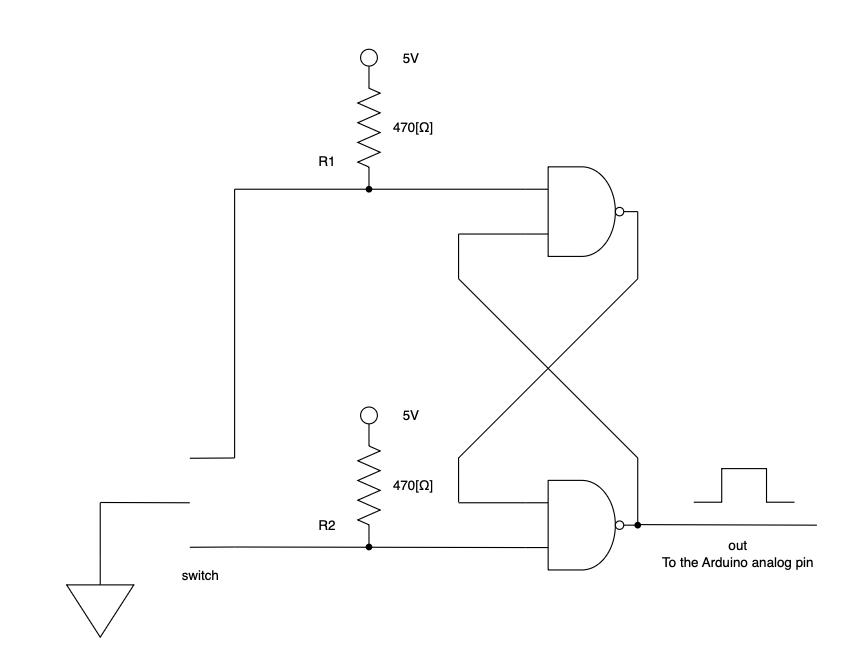
\includegraphics[width=0.7\linewidth]{fig/debounce.png}
  \end{center}
  \caption{BPM変更スイッチのチャタリング対策回路}
  \label{fig:debounce}
\end{figure}

この回路は，2つのNAND素子を交差接続したフリップフロップを用いており，スイッチが切り替わると
回路の状態が保持される．これにより，接点のバウンスによる複数回の信号変化が出力に現れず，
1回の安定した信号が得られる．出力をArduinoのディジタルピンに接続し，\texttt{digitalRead}関数で
スイッチの押下を検出する．BPM変更スイッチはアップ用とダウン用の2つが必要であるため，
この回路もそれぞれに対して実装する．

\subsubsection{サーボモータの接続}
クライアントでは，人形の可動部を駆動するためにサーボモータを用いる．サーボモータとArduinoの接続を
図\ref{fig:servo}に示す．サーボモータの信号線をArduinoのディジタル出力ピンに接続し，5Vを供給して
駆動する．受信した演奏情報に応じてサーボを動作させることで，演奏に同期した人形の動きを実現する．
図\ref{fig:servo}では，サーボモータの電源としてArduinoの5Vを使用しているが，複数のサーボモータを同時に駆動する場合は，外部電源を使用することが望ましい．
実際に，トロンボーン人形を除いたピアノ・カスタネット・ヴァイオリンの３体はそれぞれ2つのサーボモータを使用しており，Arduinoの5Vでは電流が不足するため，外部電源を使用している．
なお，図中ではサーボモータをD9ピンに接続しているが，人形の右腕をD9ピンに，左腕をD11ピンに，頭や口などはD5ピンに接続する設計となっており，
サーボモータの接続ピンは人形ごとに異なる．

\begin{figure}[H]
  \begin{center}
    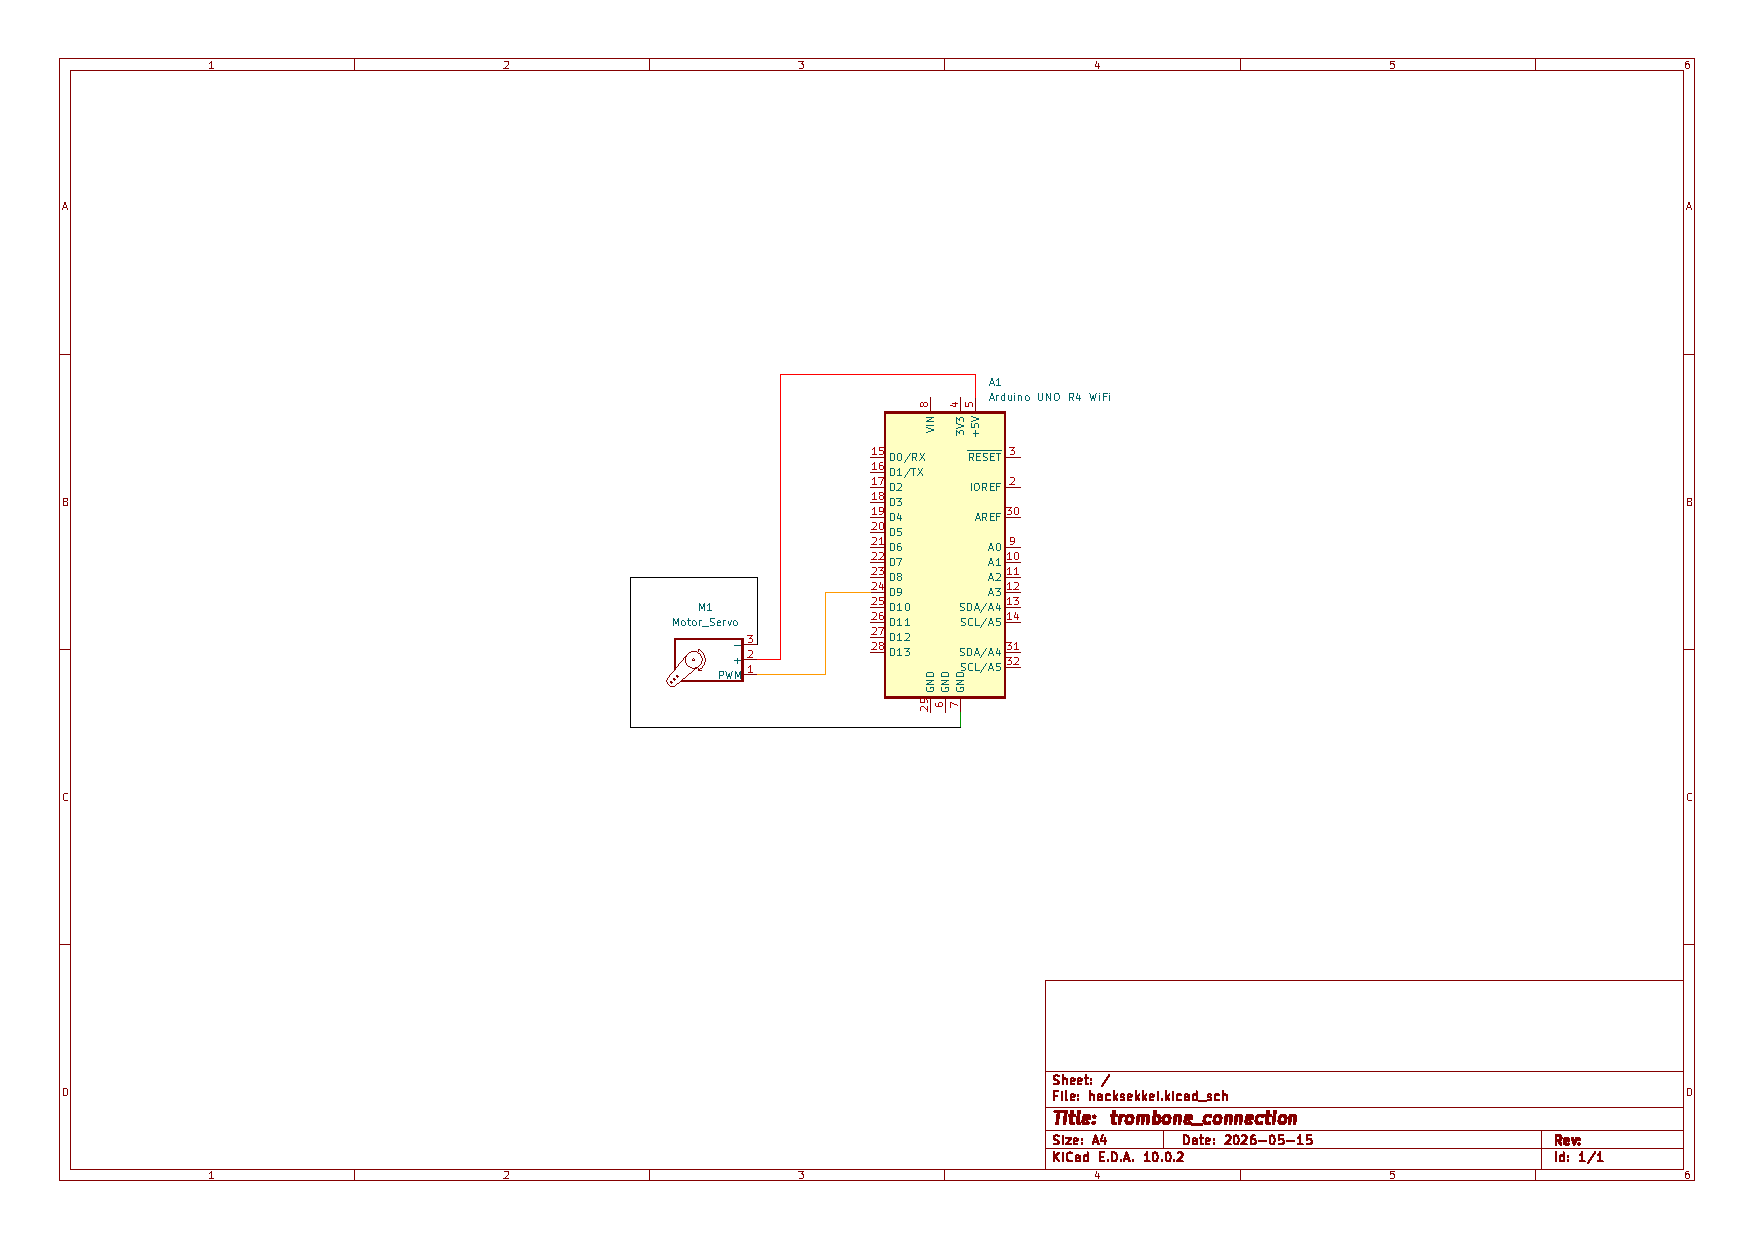
\includegraphics[width=0.7\linewidth]{fig/hacksekkei.pdf}
  \end{center}
  \caption{サーボモータを使用したクライアント部分の回路図}
  \label{fig:servo}
\end{figure}

\subsection{生成AIの活用と検証}
本開発では，音源解析に関するコードの作成に生成AIを活用した．一方で，生成AIが出力する結果は，
その処理内容を理解した上で妥当性を検証する必要がある．本節では，トロンボーンの音源設計における
生成AIの活用とその検証について述べる．

トロンボーンの音色を設計するにあたり，実際のトロンボーンの音に含まれる倍音の構成を参考にすることとした．
そこで，音源のスペクトルから倍音の振幅を抽出するFFT解析のコードの作成を生成AIに依頼し，得られた
コードを用いて解析を行った．当初はこの解析結果を倍音の振幅として波形テーブルに用いた．
しかし，後の検証において，抽出された周波数がいずれも基本周波数の近傍に集中しており，倍音を正しく
抽出できていないことが判明した．原因を確認したところ，生成されたコードはFFTの振幅を単純に大きい順に
並べるものであり，スペクトルのピークを検出する処理を含んでいなかった．そのため，倍音のピークではなく，
基本周波数の1つのピークの近傍にある複数の値を抽出していた．
この問題を踏まえ，解析コードにピーク検出処理（\texttt{scipy.signal.find\_peaks}）を導入し，
ピーク間の最小間隔と卓立度を指定することで，倍音のピークを適切に分離して抽出できるように改善した．
この経験から，生成AIが出力するコードは，処理の内容と結果の妥当性を利用者自身が確認した上で
採用する必要があることを確認した．以降の解析では，公式ドキュメントを参照しながら処理内容を
確認し，生成結果を検証した上で採用する方針を取った．

カスタネットの音源生成においては，これを踏まえて，生成AIに対してFFT解析のコードを作成する際に，ピーク検出処理を含めるように指示した．
更に，Processing上での音色再現についても，減算合成の手法を用いて，FFT解析の結果をもとに各成分の中心周波数・減衰時間・フィルタ特性を調整するコードを生成AIに作成させた．
導入する以前の音色と比較すると，明らかにより実際のカスタネットの音に近い音色が得られ，
その他の問題が発生しないことを確認し，実際のシステムに採用した．

また，楽器の単体テスト用に波形を出力し，周波数を表示するコードを生成AIに作成させ，実際の楽器音と合成音の周波数成分を比較することで，設計値の妥当性を検証した．
コードの中では，もともとinoファイルで定義されている周波数をそのまま使用しているので
正当性は担保されている．それに加え，評価で用いる自己相関法を用いた，理論周波数との相対誤差を算出するコードと，その結果をグラフ化するコードも生成AIに作成させ，
ゼロ交差法も同様に生成AIに作成させた．